\section{Method}
In this section, we first present the problem formulation. We then introduce the architecture of our model, followed by the training objectives that enable static–dynamic disentanglement and the recaching mechanism. Next, we provide a computational complexity analysis and derive the theoretical acceleration and context-length improvements. Finally, we introduce the benchmark for evaluating multi-frame integration.

\noindent\textbf{Problem Formulation}
Given a timestep $t$, the corresponding observation of the environment is denoted by $\bs{X}_t$. A VLA $\pi$ predicts actions of the following steps based on previous $T$ observations and a language instruction $\mathcal{I}$.
\begin{equation}
    \pi: (\bs{X}_{t-T}, \bs{X}_{t-T+1}, \cdots, \bs{X}_{t}, \mathcal{I}) \mapsto \bs{a}_t, \bs{a}_{t+1}, \cdots,
\end{equation}

\begin{figure}[t]
    \centering
    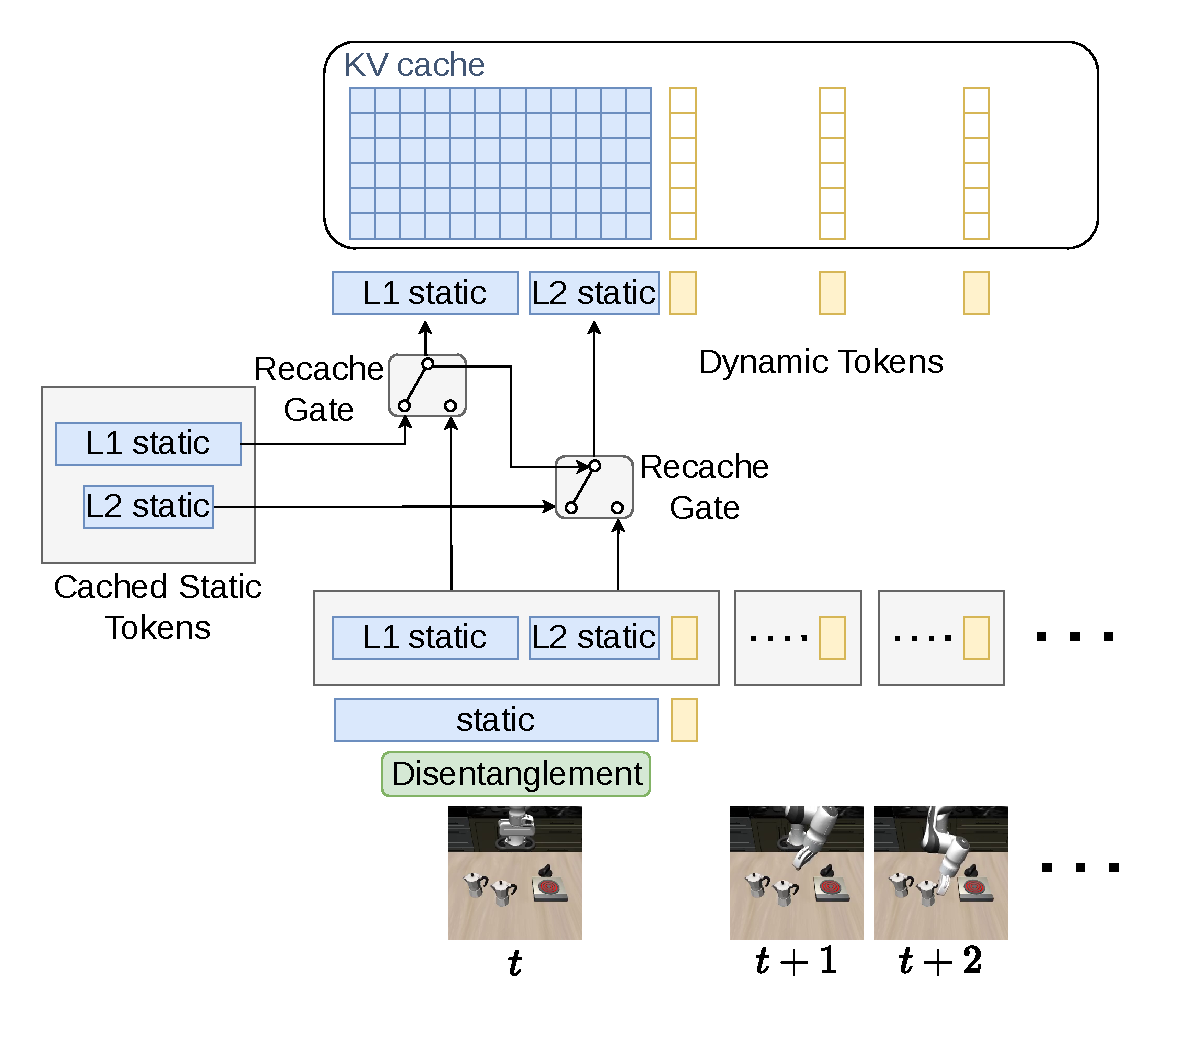
\includegraphics[width=0.9\linewidth]{figs/arch.pdf}
    \caption{Model architecture overview. We illustrate the design using two levels of static cache. At each level, a recache gate determines whether the cached static tokens should be reused or refreshed. If the L1 cache is refreshed, the L2 cache is also forcibly refreshed.}
    \label{fig:dysta-arch}
    % \vspace{-1em}
\end{figure}


where $\bs{a}_t$ is the action at the $t$ step. Most existing VLAs usually consider $T=0$ due to the limited context length of large language models.


\subsection{Model Architecture}
\noindent\textbf{Static-dynamic disentanglement}
Standard VLA vision backbones typically encode the image $\bs{X}_t$ into $N$ image tokens $\bs{Z}_t=\bs{z}_{t,1}, \bs{z}_{t,2}, \cdots, \bs{z}_{t,N}$ as inputs of the VLA's LLM backbone $\pi_\text{LLM}$. Such a design implicitly assumes that all visual tokens must be recomputed and reprocessed at every timestep. However, real-world environments exhibit strong temporal redundancy: many visual attributes remain unchanged across time, while only a subset varies dynamically. Moreover, static information exists at different temporal scales. For example, global scene layout or background structure may persist for long horizons, whereas object-level appearance may change more frequently due to occlusion or interaction. To reflect this structure, we disentangle visual tokens into multi-level static tokens and dynamic tokens.

\begin{equation}
\bs{Z}^{s_1}_t, \bs{Z}^{s_2}_t, \cdots, \bs{Z}^d_t = \\
  \underbrace{\bs{z}_{t,1}, \cdots, \bs{z}_{t,N_{s_1}}}_\text{static tokens (level 1)}, \underbrace{\bs{z}_{t,1}, \cdots, \bs{z}_{t,N_{s_2}}}_\text{static tokens (level 2)}, \cdots, \underbrace{\bs{z}_{t,1}, \cdots, \bs{z}_{t, N_d}}_\text{dynamic tokens}
\end{equation}

where $\bs{Z}^{s_l}_t$ denotes static tokens at level $l$, and $\bs{Z}^{d}_t$ are dynamic tokens. The ratio between static and dynamic tokens is set as a predefined hyperparameter. Under this design, dynamic tokens capture timestep-specific information and are recomputed at every timestep, whereas static tokens at each level are selectively reused through a learned caching mechanism, described later.

\noindent\textbf{Temporal dependency modeling}
Most VLAs \cite{kim2024openvla,li2024cogact,qu2025spatialvla} are only able to process the current observation ($T=0$),
\begin{equation}
    \bs{a}_t, \bs{a}_{t+1}, \cdots = \pi_\text{LLM}(\bs{Z}_t),
\end{equation}
where $\pi_\text{LLM}$ is the LLM backbone of the VLA.
With successful static-dynamic disentanglement, we only need to keep \emph{one copy} of the static tokens within a period and construct the input from multiple observations as

\begin{equation}
    \bs{a}_t, \bs{a}_{t+1}, \cdots = \pi_\text{LLM}(\bs{Z}^{s_1}, \bs{Z}^{s_2}, \cdots,\bs{Z}^d_{t-T}, \cdots, \bs{Z}^d_t),
\end{equation}

This formulation enables the model to leverage longer temporal context without duplicating static information, effectively alleviating context window bottlenecks while preserving relevant visual cues.

\noindent\textbf{Learning when to recache}
A key challenge is deciding when cached static tokens should be refreshed. Naively recomputing static tokens at every timestep negates any computational benefit, while overly aggressive reuse of static tokens risks stale representations. To address this, we introduce a learned recache gate at each static level $l$,

\begin{equation}
    g_l(\bs{Z}_{t-\Delta}, \bs{Z}_t) \in [0, 1],\quad \Delta=1,2,\cdots, 
\end{equation}

which predicts the probability that static tokens should be recomputed given the current observation and a cached reference from $\Delta$ timesteps earlier. During training, we use the Gumbel-softmax trick \cite{jang2016categorical,maddison2016concrete} to allow end-to-end differentiable binary decisions. At inference time, static tokens are refreshed if the probability is greater than a threshold, i.e., $g_l > \delta_l$; otherwise, the previous cache is reused. It is also worth noting that if the higher-level cache (e.g., L1) should be refreshed, the lower-level cache (e.g., L2) should also be refreshed during both training and inference. Additional details of the architecture of the recache gate could be found in Appendix~\ref{app:arch}.


\noindent\textbf{Computational and Acceleration Analysis}
Let $N$ be the total number of tokens per observation, $r$ the fraction of cached static tokens, and $T$ the number of observations in the context. Our static-dynamic disentanglement reduces the effective context length from $NT$ to $NT - rN(T-1)$, and reduces the FLOPs of the LLM backbone by a factor of $1-r$. The recache gate adds only negligible overhead ($\approx 1.27\%$). A full derivation and wall-clock latency breakdown are provided in Appendix~\ref{app:complexity}.

\begin{figure}[t]
    \centering
    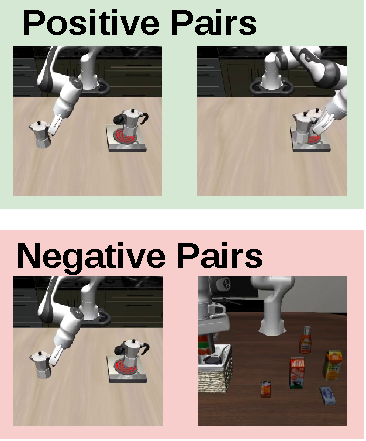
\includegraphics[width=0.5\linewidth]{figs/contrastive.pdf}
    \caption{Contrastive loss used to train static tokens to be temporally persistent. Observations from the same trajectory form positive pairs, while observations from different trajectories form negative pairs.}
    \label{fig:contrastive}
    % \vspace{-1em}
\end{figure}

\subsection{Training Objective}


Besides the standard task loss of the underlying VLA base model $\mathcal{L}_\text{task}$, we introduce two additional training objectives. The first promotes temporally persistent static tokens, and the second trains the cache gate that adaptively determines when cached representations should be refreshed.

\noindent\textbf{Learning static tokens} As illustrated in Figure~\ref{fig:contrastive}, to ensure that static tokens can be safely and effectively reused across time, they must remain stable over a temporal window while still encoding task-relevant information. To encourage this property, we apply a contrastive term to the static tokens. Specifically, observations from different timesteps within the same trajectory are treated as positive pairs, while observations from different trajectories are treated as negative pairs. We employ InfoNCE loss~\cite{oord2018representation} $\mathcal{L}_{\text{InfoNCE}}^{l}$ to perform contrastive learning for static tokens at level $l$.



% \begin{equation}
% \begin{aligned}
%     &\mathcal{L}_\text{InfoNCE}^l= \\
%     &\frac{1}{TN_{s_l}} \sum_{\Delta=1}^T \sum_{i=1}^{N_{s_l}} \frac{\exp(\bs{z}^{s_l}_{t,i} \cdot \bs{z}^{s_l}_{t-\Delta, i})}{\exp(\bs{z}^{s_l}_{t,i} \cdot \bs{z}^{s_l}_{t-\Delta, i}) + \sum_{z^-}\exp(\bs{z}^{s_l}_{t,i} \cdot \bs{z}_{}^-)},
% \end{aligned}
% \end{equation}
% where $N_{s_l}$ is the number of static tokens at level $l$. $\bs{z}^-$ are negative samples (i.e., observations from different trajectories). 

% Optimizing this objective encourages static tokens to remain consistent across timesteps within a trajectory, thereby making cache reuse safer and more effective during inference.

\noindent\textbf{Training the recache gate}
If the recache gate is trained only through task supervision, it tends to recompute static tokens at every timestep, which eliminates any computational benefit. To discourage this trivial solution, we add a regularization term that biases the gate toward reuse when observations are close in time.

\begin{equation}
    \mathcal{L}_\text{gate} = -p_\Delta \log g - (1-p_\Delta)\log (1-g),
\end{equation}

where $p_{\Delta} = 1 - e^{-\lambda \Delta}$ is a predefined prior which allows the use of current observation only when $\Delta$ is large. The recache gate learns to adaptively refresh static tokens only when necessary, balancing computational efficiency and model performance. Note that since $\lambda$ and the recache threshold $\delta_l$ jointly determine the recaching frequency, we fix $\lambda$ and expose only $\delta_l$ as the operating-point knob. 

The full training objective is
\begin{equation}
    \mathcal{L} = \mathcal{L}_\text{Task} + \sum_l \alpha_l  \mathcal{L}^l_\text{InfoNCE} + \beta \mathcal{L}_\text{gate},
\end{equation}
where $\alpha_l$ and $\beta$ weight the auxiliary regularization terms. A sensitivity analysis for these coefficients is provided in Appendix~\ref{app:sense}.

\subsection{LIBERO-Memory Benchmark}

Existing VLA simulation benchmarks \cite{liu2023libero, li2024evaluating} are designed for memoryless tasks, which do not require multi-frame integration, and the current observation alone is theoretically sufficient to predict the next action. For example, in a task with the goal “put X in the basket”, \cite{liu2023libero} the agent can act optimally without retaining information from previous frames. As a result, it is unclear whether the reported performance of existing models for modeling temporal dependency \cite{jang2025contextvla,shi2025memoryvlaperceptualcognitivememoryvisionlanguageaction} truly stems from improved temporal modeling or from other artifacts. This highlights the absence of a strong and fair benchmark for temporal dependency modeling and multi-frame integration.

To address this gap, we introduce a new simulation benchmark designed to test multi-frame integration explicitly. Our benchmark includes tasks that require a robot to retain and utilize information from past observations, thereby directly evaluating a model's temporal dependency modeling ability.

Following the setup of LIBERO, the robot operates in a tabletop environment containing three objects: two visually distinct cans and a stove. As illustrated in Figure~\ref{fig:libero_stove}, each episode consists of three tasks which reflects the structure of episodic memory \cite{tulving1972episodic,clayton1998episodic}.

\begin{figure}[t]
    \centering
    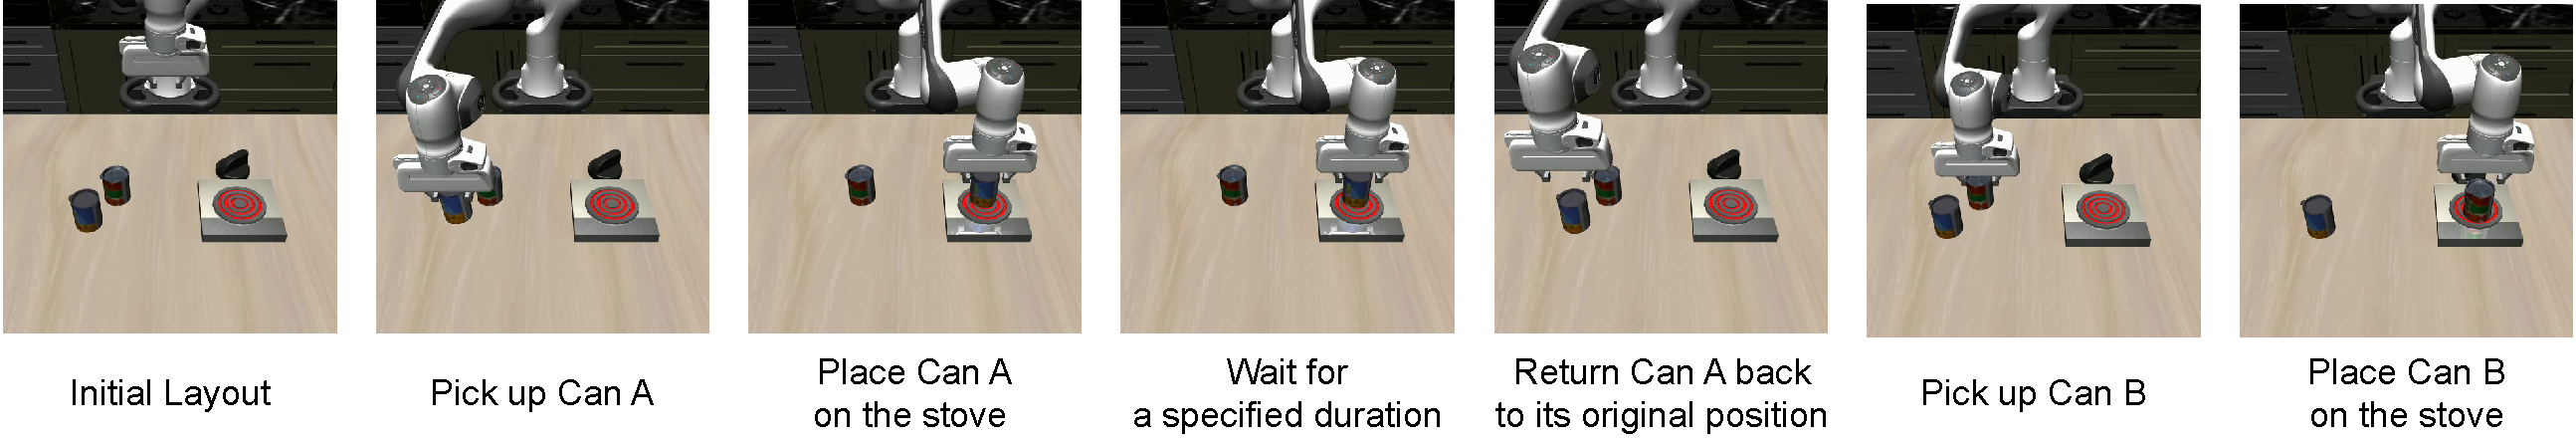
\includegraphics[width=\linewidth]{figs/libero_stove.pdf}
    \caption{An example of the procedure of the proposed benchmark. }
    \label{fig:libero_stove}
    % \vspace{-1em}
\end{figure}


\noindent\textbf{Tasks}
Each trial consists of three subtasks, each intentionally designed to require the model to retain and reason over information from previous observations at different aspects: 1) Grasp one of the cans, as specified by the instruction, and place it on the stove to heat. 2) After a period of time (given in the instructions), remove the can from the stove and return it to its original location. 3) Once the position of the first can has been restored, grasp the remaining can and place it on the stove.

This task design requires the model to retain \emph{episodic memory}, integrating information about what happened, where it occurred, and when it took place \cite{tulving1972episodic,clayton1998episodic}. First, the robot must remember the initial spatial layout in order to return the first can to its original position (where). Second, it must track the elapsed time since the can was placed on the stove to determine when to remove it (when). Third, it must remember which can has already been heated in order to correctly select the remaining one for the final step (what).

These requirements prevent the task from being solved using only the current observation or a short observation history. We use Robosuite \cite{zhu2025robosuitemodularsimulationframework} as the simulation framework to produce the dataset. The layout and the oracle demonstrations are programmatically generated. More details can be found in Appendix \ref{app:dataset_memory}.
